%This is my super simple Real Analysis Homework template

\documentclass{article}

%% Language and font encodings
\usepackage[T1,T8K,T8M]{fontenc}
\usepackage[utf8]{inputenc}
\usepackage[english,georgian]{babel}

\usepackage{amsmath}
\usepackage{graphicx}
\usepackage[colorinlistoftodos]{todonotes}
\usepackage[colorlinks=true, allcolors=blue]{hyperref}
\usepackage{float}
\usepackage{enumerate}
\usepackage{subfig}
\usepackage{gensymb}

%\title{დავალება 01}
%\author{Your Name}
%\date\today
%This information doesn't actually show up on your document unless you use the maketitle command below

\begin{document}
%კომაროვის მერვე კლასის წრე 2016წლის 11 დეკემბერი
\subsection{ამოცანა 1}
$N = 600$ ვტ სიმძლავრის ელექტრული ნათურა ჩაუშვეს გამჭვირვალე კალორიმეტრში, რომელშიც $m = 600$ გ წყალი ასხია. $\tau = 5$ წუთში წყალი გათბა $\Delta t = 46 C \degree$-ით. ენერგიის რა $k$ ნაწილი გამოასხივა კალორიმეტრმა? წყლის კუთრი სითბოტევადობა $c = 4.2 \cdot 10^3$.

\subsection{ამოცანა 2}
$10 C \degree$ ტემპერატურის წყალში $100 C \degree$ ტემპერატურის სხეულის ჩაშვების შემდეგ დამყარდა $40 C \degree$-ის ტოლი საერთო ტემპერატურა. როგორა შეიცვლება წყლის ტემპერატურა, თუ პირველ სხეულს წყლიდან არ ამოვიღებთ და ჩავუშვებთ $100 C \degree$ ტემპერატურის ისეთსავე მეორე სხეულს.

\subsection{ამოცანა 3}
ცილინდრულ ჭურჭელში ჩასხმული ზეთის ზედაპირზე დაცურავს ყინულის ნაჭერი. როგორ შეიცვლება წნევა ფსკერზე და ზეთის დონე ჭურჭელში, როდესაც ყინული მთლიანად გადნება და წარმოქმნილი წყალი დაეშვება ჭურჭლის ფსკერზე?

\subsection{ამოცანა 4}
1 მ სიგრძის მოხრილი მილი ავსებულია წყლით. მილის ქვედა ბოლო დაცობილია და მილიდან წყალი არ გამოედინება. რა მოხდება, თუ მილის ქვედა $C$ ბოლოს გავხსნით?
	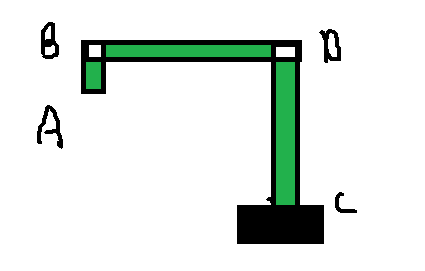
\includegraphics[scale=0.4]{figures/problem_4}
	
\subsection{ამოცანა 5}	
მოსწავლე ვასია ატარებს ექსპერიმენტს ფიზიკაში, ხოლო ძმა პეტია ეხმარება. ვასიამ ქილაში ჩაასხა $t_1 = 20 C \degree$, $V = 1$ ლიტრი მოცულობის წყალი და მოათავსა $P = 1$ კვტ. სიმძლავრის მადუღარა, ჩართო და მეზობელ ოთახში გავიდა კლასელთან ტელეფონზე სასაუბროდ. $\tau = 5$ წთ-ის შემდეგ დაბრუნდა, ქილაში წყლის ტემპერატურა გაზომა და მიიღო $t_2 = 60 C \degree$. ამავდროულად აღმოჩნდა, რომ თურმე ძმას სანამ ვასია საუბრობდა მადუღარა ცოტა ხნით გაუთიშავს. რამდენი ხანი გრძელდებოდა ძმის დახმარება? წყლის სითბოტევადობაა $c = 4.2 \cdot 10^3$, წყლის სიმკვრივე $\rho = 1 \cdot 10^3$ . მადუღარის, ქილის სითბოტევადობა და ასევე სითბოს დანაკარგები უგუბელყავით. 

\end{document}